\section{Slow Feature Analysis (SFA)}
\textbf{Slow Feature Analysis (SFA)}\index{Slow Feature Analysis (SFA)} とは, 複数の時系列データの中から低速に変化する成分 (slow feature) を抽出する教師なし学習のアルゴリズムである (Laurenz Wiskott, Berkes, Franzius, Sprekeler, & Wilbert, 2011; L. Wiskott & Sejnowski, 2002).

潜在変数 $y$ の時間変化の2乗である $\left(\frac{dy}{dt}\right)^2$を最小にするように教師なし学習を行う.初期視覚野の受容野や格子細胞・場所細胞などのモデルに応用がされている (Franzius, Sprekeler, & Wiskott, 2007).

生理学的妥当性についてはいくつかの検討がされている.(Sprekeler, Michaelis, & Wiskott, 2007)ではSTDP則によりSFAが実現できることを報告している.ただし,in vivoにおけるSTDPの存在については近年疑問視されている.これまでのin vitroでの実験は細胞外Ca濃度が高かったために、pre/postのスパイクの時間差でLTD/LTPが生じるという「古典的STDP則」が生じていた可能性があり,細胞外Ca濃度をin vivoの水準まで下げると古典的STDP則は起こらないという報告がある (Inglebert, Aljadeff, Brunel, & Debanne, 2020).古典的な線形Recurrent neural networkでの実装も提案されている ([Lipshutz, Windolf, Golkar, & Chklovskii, 2020](https://arxiv.org/abs/2010.12644)).
\lstinputlisting[language=julia]{./text/local-learning-rule/slow-feature-analysis/001.jl}
\subsection{SFAの前処理}

SFAの前処理として多項式展開(polynomial expandsion)が用いられる ([Berkes & Wiskott, 2005](https://jov.arvojournals.org/article.aspx?articleid=2192836)).Pythonにおいては[sklearn.preprocessing.PolynomialFeatures](https://scikit-learn.org/stable/modules/generated/sklearn.preprocessing.PolynomialFeatures.html)により使用できる.
\lstinputlisting[language=julia]{./text/local-learning-rule/slow-feature-analysis/003.jl}
時間的にずらして時系列データの次元を増やす前処理も行われる.
\lstinputlisting[language=julia]{./text/local-learning-rule/slow-feature-analysis/005.jl}
## データセットの生成
\lstinputlisting[language=julia]{./text/local-learning-rule/slow-feature-analysis/007.jl}
\lstinputlisting[language=julia]{./text/local-learning-rule/slow-feature-analysis/008.jl}
\begin{figure}[ht]
	\centering
	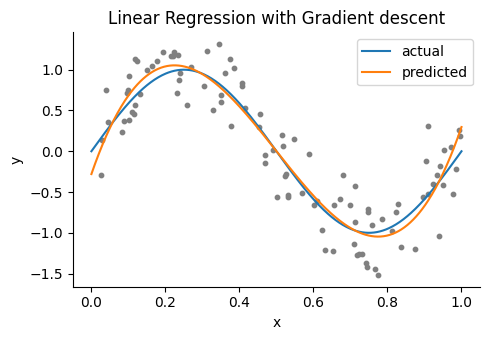
\includegraphics[scale=0.8, max width=\linewidth]{./fig/introduction/linear-regression/cell008.png}
	\caption{cell008.png}
	\label{cell008.png}
\end{figure}
## SFAの実装
\lstinputlisting[language=julia]{./text/local-learning-rule/slow-feature-analysis/010.jl}
## 実行と結果表示
\lstinputlisting[language=julia]{./text/local-learning-rule/slow-feature-analysis/012.jl}
\lstinputlisting[language=julia]{./text/local-learning-rule/slow-feature-analysis/013.jl}
\begin{figure}[ht]
	\centering
	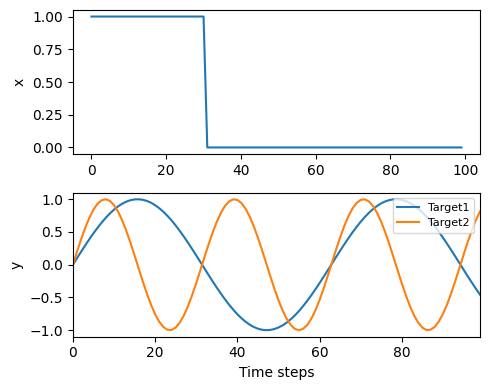
\includegraphics[scale=0.8, max width=\linewidth]{./fig/solve-credit-assignment-problem/bptt/cell013.png}
	\caption{cell013.png}
	\label{cell013.png}
\end{figure}
\subsection{参考文献}
\begin{itemize}
\item \url{https://towardsdatascience.com/a-brief-introduction-to-slow-feature-analysis-18c901bc2a58}
\item \url{https://github.com/flatironinstitute/bio-sfa}
\item \url{https://github.com/fulviadelduca/slow-feature-analysis}
\item [Deep Slow Feature Analysis Network](https://github.com/rulixiang/DSFANet)
\item \url{https://nbviewer.jupyter.org/github/pierrelux/notebooks/blob/master/Slow%20Feature%20Analysis.ipynb}
\end{itemize}
